\documentclass[conference]{IEEEtran}
\IEEEoverridecommandlockouts
% The preceding line is only needed to identify funding in the first footnote. If that is unneeded, please comment it out.
\usepackage{cite}
\usepackage{amsmath,amssymb,amsfonts}

\usepackage{graphicx}
\usepackage{textcomp}
\usepackage{xcolor}
\usepackage{algorithm} 
\usepackage{algpseudocode} 
% Emad Added the bellow packages
\usepackage{todonotes}

\def\BibTeX{{\rm B\kern-.05em{\sc i\kern-.025em b}\kern-.08em
    T\kern-.1667em\lower.7ex\hbox{E}\kern-.125emX}}
\begin{document}


\title{Distinct Clause on Find Usages}



\author{\IEEEauthorblockN{Emad Aghayi}
\IEEEauthorblockA{\textit{Department Of computer Science} \\
\textit{George Mason University}\\
Fairfax, VA \\
eaghayi@gmu.edu}
\and
\IEEEauthorblockN{Aaron Massey}
\IEEEauthorblockA{\textit{Department Of computer Science} \\
\textit{George Mason University}\\
Fairfax, VA \\
amassey5@gmu.edu}
\and
\IEEEauthorblockN{Thomas LaToza}
\IEEEauthorblockA{\textit{Department Of computer Science} \\
\textit{George Mason University}\\
Fairfax, VA \\
tlatoza@gmu.edu}
% \and
% \IEEEauthorblockN{3\textsuperscript{rd} Given Name Surname}
% \IEEEauthorblockA{\textit{Department Of computer Science} \\
% \textit{George Mason University}\\
% Fairfax, VA \\
% email address or ORCID}
}

\maketitle

\begin{abstract}
Developers face many challenges when trying to understand large codebases. In particular, they have difficulties in understanding the context of how various internal classes, objects, or methods are used in the codebase. We sought to better understand these challenges by conducting a think-aloud user study with 6 participants. The results of the think-aloud experiment highlighted that developers spend considerable time learning to use internal code artifacts. The result also showed developers use the Find Usages/References feature of IDEs to understand code by example. The results of find usage can be long tail of results that developers find difficulty mentally parsing. We also found that find usage/reference results' would contain duplicate examples in disparate locations in the UI, adding to the difficulty of parsing. Based on the think-aloud study, we hypothesized that removing duplicate examples and grouping similar examples together would reduce the excise in using the find usages/references tool. We designed and implemented a plugin for IntelliJ IDEA that manipulated result of find usages and grouped them based on their similarity. After that, we conducted a controlled experiment with 10 more participants to evaluate our approach. Results showed that this aggregation of unique examples is useful.
\end{abstract}

\begin{IEEEkeywords}
Code navigation, information foraging, Find Usages, Find References, large Codebase
\end{IEEEkeywords}

\begin{figure}
    \centering
    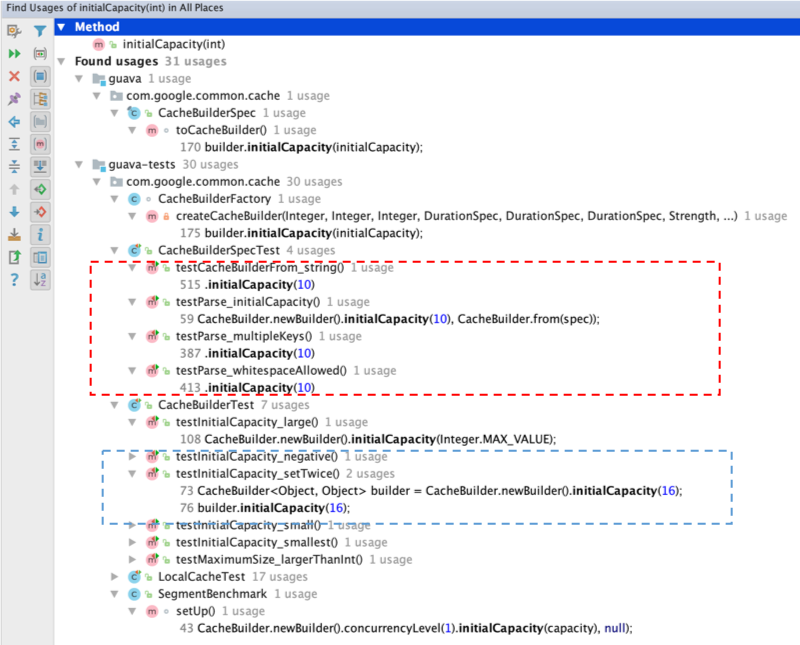
\includegraphics [width=\columnwidth,keepaspectratio, clip]{figures/Picture1}
    \caption{It depicts result of Find Usages of IDE. The result window shows there exist 31 usages of the ‘initCapacity’ method. Developers have to go through all of 31 results and also use a pen and paper to find the possible inputs for this method. In this 31 results many of them set same input values of this method, for example 10 is repeated multiple times. This duplicate result is annoying and time consuming for Developers. 
}
\label{fig:usege}
\end{figure}

section{INTRODUCTION}
Developers are facing many challenges every day for understanding codebase. They have difficulties in understanding the context of how members are used, for instance, how object A is used in the codebase. Another daily issue is navigation from one statement other to task-related code. Sometimes developers want to go through related statements to understand the codebase. Also, they are facing challenges to answer questions about how a change affects callers when developers want to change an artifact before changing that they check the side effect of that change. They go through the codebase and evaluate the effect of change on them. There exist multiple approaches for better support of structural navigation.\par
During programming tasks, it is not uncommon for a developer to use an object or routine they were previously unfamiliar with. A programmer could also be unfamiliar with how a resource is used within a codebase versus the resource itself. Typically, programmers scour the web for documentation or examples~\cite{brandt2009two}. However, this is not an option for closed source code, forcing developers to rely on internal documentation and examples. Since this may be non-existent or worse (incorrect), example code is a more reliable information source for programmers. The industry-standard approach for finding examples is the Find Usages/References tool. However, when large numbers of references are returned from this tool, it can be not very easy for users to parse the results visually .\par
We conducted an exploratory study to find are challenges of understanding codebase while developers are trying to use the Find Usages feature of IDEs. During an exploratory user study, participants would get overwhelmed with the number of results and that instead of investigating more usages, participants would select a single usage and use it as a particular example for quite some time before moving on to find other potentially better examples.
We hypothesized that some intelligent aggregation of the results would make these results easier to parse, thus improve programmer task time.\par
Based on the result of exploratory study, we created and evaluated a plugin for addressing the issues that we found. The results of our evaluation provide design insights that have implications for future researches.\par


\section{Relate Work}
Developers are using code navigation in their daily activities. For instance, they want to want to understand what a method does or when it is called or want to understand how to reuse a function by finding examples of code snippets. They investigate source code. Navigating in source code is described in information foraging theory~\cite{pirolli1999informationforaging}. In software engineering, this theory usually modeled as call graphs. Methods are nodes, and function invocations are edges. Developers have challenges in traversing the call graph in code navigation~\cite{albusays2017interviews}. Navigating and re-finding place of the code that had already been visited was frequent, difficult and distracting~\cite{ko2005eliciting,deline2005towards}.\par 

Tools are trying to help developer to be more productive in the code navigation. These tools are grouped into three categories. The first category is structural relationship traversal. These tools find starting point then traverse relationships to find other related code locations~\cite{karrer2011stacksplorer,augustine2015field,latoza2011visualizing}. Another category is recommender tools. Based on history developers did on similar tasks, they predict relevant elements~\cite{zimmermann2005mining,deline2005easing}. Task context navigation is the last category of code navigation tools. They make it easier to navigate back and forth between task context elements~\cite{ko2006exploratory}. Although there exist several tools for code navigation, code navigation is still challenging for developers~\cite{albusays2017interviews}. 

A common way to edit code is by copying existing code, called code clones~\cite{codeCloneDetection2019}. Sometimes code clone is bad, but there exist many situations that code clone is fine. Developers, because of reasons like basic template, design patterns, or reuse of the definition of specific behavior, use code clones~\cite{kim2004ethnographic,kapser2008cloning}. There exist many tools for detecting code clones in codebases~\cite{bellon2007comparison}.\par 

There is a plethora of research on information foraging and improving learning by examples~\cite{brandt2009two}. There is also much work in code clones code clone clustering~\cite{codeCloneDetection2019}. As far as these authors are aware, this is the first time work on code clones, and their clustering has been used to help forage for examples within a codebase. Typically code cloning is used to infer duplicate code snippets for refactoring or patching. Researchers have attempted to take relevant pieces from each of these fields, and it is this combination of parts that is the contribution~\cite{kapser2009toward}.\par


Find a similar code in a codebase is one code reuse strategy~\cite{rosson1996reuse}. Developers looking for examples of how to use specific methods or objects~\cite{stylos2006mica,umarji2008archetypal}. Opportunistic developers more likely to use example code rather than systematic developers. There exist techniques for supporting reuse, for instance, IDEs has searching feature that enables developers to search for example across the existing codebase, or IDEs has feature for fining right sequence of methods to complete some tasks that developer already started.\par

Developers, when they write or edit code, they might come across code element that they want to change or delete. Before they make changes, they look where the code element is used and how it affects the codebase. \textit{Find Usages} feature in Jetbrains IDEs and \textit{Open Call Hierarchy} feature of Eclipse Provided this ability for developers. Results of Find Usages are listed in window in Jetbrains IDEs that developers are going through the results to find the desired usage or understand the codebase. 
\todo[inline]{add challenge of Find usages}
\par



\section{Challenges and Benefits of Understanding Codebase}
We conduct a think-aloud study to understand better current practice and the challenges developers face using existing approaches. The study was in-person, and their interaction and thoughts were recorded. Researchers vocally recorded the process while asking the participant to think-aloud while conducting the study. The participants were allowed to ask for hints or questions or clarifications, but we must not give answers.
We were not looking for successful implementation. We were looking for what developers think about the find usage interface, without coaxing the answers we may want out of them.
We recruited four participants (P1, P2, P3, P4), two female and two male. The first participant was a graduate computer science student at George Mason University. The remaining three participants were working as a software developer in the industry, two of them had experienced less than one year, but one of them had more than four years of experience in the industry. We designed two tasks for the study. In the beginning, the tasks were piloted with the graduate student participant to make sure the tasks are designed correctly or not. At the and of study, we asked participants to respond to a survey for collecting their experience. In that survey, we asked them 1)What challenges did they experience related to finding a method, variable, or anything. 2)What challenges, if any, did they experience as they tried to begin work l on these tasks? 3)What challenges, if any, did they experience related to understanding and working with the provided codebase?   4) What challenges, if any, did they experience related to their productivity? 

\subsection{Tasks of Exploratory Study}

The first task was a warm-up for using a find usages tool for code comprehension. The codebase that participants worked on it was Google Guava (772,475 LOC), an open-source set of standard libraries for Java. We chose this library because we thought it is standard and is large enough. We gave the participant a zip file that contained the Guava and asked them to qualitatively describe the range of integer inputs given to the two methods. We gave participants to work on firs task on any IDE that they are more familiar with. Time of the first task was 10 minutes.\\
Since we also wanted to understand the behaviors of developers when they are trying to change a codebase, we designed second task for developers. The codebase that we chose for this task was FlyingSaucer, pure Java library for rendering XML, XHTML, and CSS. It was a large codebase 99,000 LOC. We removed statements that create PDF from the codebase, then asked participants to implement functionality to produce “success.pdf.” We added a constraint on the task. Participants should treat code as closed source code, meaning they cannot find JavaDocs online or look for online code examples, but they were free to choose any IDE for accomplishing the task. The study was in person, and it lasts 50 minutes for each participant. 

\subsection{Results of Exploratory Study}

\todo[inline]{Write a qualitative description of the short exercises and what was done. Like how only the senior dev was familiar with the find usages tool.}

We collected data from the interaction of developers while they were working on both tasks. During the first task, participants clicked through multiple usages trying to understand how certain common arguments to methods were called. We have participants a maximum of 10 minutes to feel like they had become comfortable with the find usages tool. Participants completed task two in 49, 20, 42 minutes. Two participants had a problem with the size of the codebase.
\begin{quote}"Overwhelmed by the amount of code." - (P2) \end{quote}
\begin{quote}"Large codebases are my biggest fear." - (P4) \end{quote}
3 of 4 did not know about the Find Usage feature, which was interesting. We gave them information and train them what is Find Usage feature and how they can use it. One of them Used the term "implemented" to mean "usage" frequently. In some cases, participants did not have a strong evidence or reason for understanding the codebase. They were trying to use their feeling. 
\begin{quote}"I donot know how .layout() is used but I am going to use it because it's in this code" - (P2) \end{quote}
\begin{quote}"I feel like this [.layout()] should just work, I hope!" - (P4) \end{quote}

Tasks that we defined looked was similar to what they are doing in their job in the industry. 
\begin{quote}
"Not out of the ordinary [from regular industry/work experience] but still a bit overwhelming"- (P2)
\end{quote}
\begin{quote} "This is just like my job" and "I do this at work all the time, no one knows how anything works but we see how things are used"
- (P3)
\end{quote}
The codebase that we gave participants included unit tests. The interesting thing was that participants were using these unit tests to figure out how methods are invoked and what are the possible input arguments for those methods. They primarily utilized tests as examples. Participants sticks to the specific test case, and usage found, do not go looking for others much until it gets too complex of a usage.

\begin{quote} "Tests are a good example of uses." - (P3)\end{quote}

The similarity of Find Usages results was a severe issue for the participants since the codebases were reasonably large participants while were trying to use the Find Usages feature. The IDE was returning many results, which was challenging for participants to extract useful information for undressing the method or object. When doing find usage, much code looked similar, and it was difficult for the participant to parse for participants. Also, this problem was severe when the method they tied to get Find usage was complex and had complicated call graphs.

\begin{quote}"There were a ton of methods and usages that were really similar and it was a lot to put together"- (P4)\end{quote}
\begin{quote}"I had difficulty finding usages with low complexity of calls and uses"- (P4)\end{quote}

Another typical behavior was that participants were Scrolling quickly through usages because the surrounding code was not making calls she wanted to make. Participants occasionally navigated to unhelpful usages that took time. A surprising behavior as participants focused on the first result of Find Usage, they copied the first usage, then paste it into the place they want to implement and tried to change it in the way they want. The confusing thing about Find Usage is happen when a method is overloaded. Participants had difficulty migrating to the correct find usage because of overloaded methods.


\section{FIND UNIQYE USAGE METHOD}
Result of the think-aloud study revealed there exist challenges in using Find Usages feature, participants overwhelmed with tons of usage, and they spent much time in going throw many of them for understating the codebase. We brainstormed on the results and came up with the idea that the refining result of Find Usage might help developers and increase their productivity. In order to create a better tool for addressing the issues, we must understand what is going on in the developers' world and understand how our tool can make the developers' productivity higher. Therefore, we summarized research findings into storyboards. We designed a plugin for IntelliJ IDEA that refines the result of the Find Usages feature. In our tool that we named it Find Uniques Usages (FUU) works similar to DISTINCT command in SQL language, the main idea of FUU in SQL language is \begin{verbatim} SELECT DISTINCT usages FROM Codebase \end{verbatim}. It aggregates the results and shows the only relevant results. Relevant results likely depend on a measure of sameness.\par

\todo[inline]{we need to find better usages tool for readers unfamiliar with the ide and this part of it.}

\todo[inline]{Below section needs two screenshots to compare, one of the classic find usages and another of our extension.}

The basic idea behind Find Unique Usages is to group results from a standard Find Usages/References IDE operation based on each result's surrounding code.
\begin{figure}
    \centering
    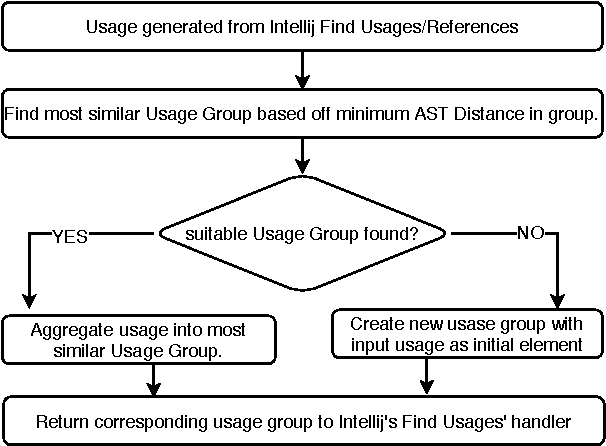
\includegraphics [width=\columnwidth,keepaspectratio, clip]{figures/flowchart}
    \caption{XYZ. 
}
\label{fig:usege}
\end{figure}

\subsection{User Interface} 
% We may need an extra description of the pre-existing user interface
Because the adoption of new tools and UIs can be onerous to programmers (needs citation?). We extended the existing Find Usages interface of IntelliJ by adding additional usage groups that contained usages with similar code. Since each user group contained usages that were surrounded by similar code, we hypothesized the usages would be in similar contexts, implying more information about the usage. So a user could inspect one usage within a usage group and gleam that the other usages within that group were similar and move on to another usage group depending on their task. The task we associate this tool with is finding and parsing a large variety of usages while seeking examples of an internal API.

\subsection{Usage Grouping Backend} 
Usages were grouped based on similar code within the usage's containing method code block. \todo[inline]{let's use a highlighted example with colors here maybe?} For every usage, Intellij calls our aggregate usage method, which returns a reference to a particular UsageGroup, an internal IntelliJ object representing groups of usages. We compare the given usage with all other usages in all existing usage-groups. We consider the given usage to be a part of a usage group when it has a guaranteed minimum threshold of similarity with every AST associated with that usage-group. If all the USageGroups have minimum similarities that do not meet the threshold, then we create a new UsageGroup with the supplied usage and then return that UsageGroup. This is a naive approach to clustering that we took due to time constraints preventing us from better understanding the Intellij SDK. In the future, we hope to reimplement the usage grouping with merging as part of an agglomerative clustering approach.

\subsection{AST Diffing}
We used ~\cite{spoonlabs_2019,falleri2014fine}, which leverage the GumTreeDiff algorithm. We chose this approach because GumTreeDiff is focused on fine-grained differentiation that is more sensitive to a programmer~\cite{falleri2014fine}. The gumtree-spoon-ast-diff API leverages this algorithm while providing more detailed parsing of Java source code. The authors of GumTreeDiff focus on its use in SCM, where we leverage it for grouping potential example code.


\subsection{Approach}
Our approach was to group usages found by the Intellij usage finder and group them based on similar ASTs while presenting the result to the user. Our comparison leveraged the Gumtree Spoon AST Diff framework, where we measured the resulting differing and matching nodes from an object representing the diff. 


\todo[inline]{we need a schematic to convey the concept of FUU, Emad can do it with Omnigraffle }

\begin{algorithm}
    \caption{Similarity of two Usages - similarity($x$, $y$)} 
    \begin{algorithmic}[1]
    \State $xAST$  $\leftarrow$ astOfContainingFunction($x$)
    \State $yAST$ $\leftarrow$ astOfContainingFunction($y$)
    \State // Get matching AST Nodes in common using gumtree-spoon-ast-diff
    \State $mappings$ $\leftarrow$ getMappingSet($xAST$, $yAST$)
    \State 
    \textbackslash \textbackslash  Use formula from     
    \State 
    \textbackslash \textbackslash http://leodemoura.github.io/files/ICSM98.pdf
    \State $similarity$ $\leftarrow$
    $$\frac
    {2*size(mappings)}
    {2*size(mappings) + size(xAST) + size(yAST)}$$
    \State return $similarity$
    \end{algorithmic} 
\end{algorithm}
\begin{algorithm}
    \caption{Minimum Similarity in a Usage Group - minSimilarity($x$, $G_{i}$)} 
    \begin{algorithmic}[1]
    \State Given a Usage $x$ and a Usage Group $G_{i}$
    \If{$G_{i}$ = null}
    \State return  $-\infty$
    \EndIf
    \State $minSimilarity$ $\leftarrow$ $\infty$
    \For{each usage $u_{i}$ in $G_{i}$}
    \State $minSimilarity$ $\leftarrow$ min($minSimilarity$, similarity($x$, $u_{i}$))
    \EndFor
    \State return $minSimilarity$
    \end{algorithmic} 
\end{algorithm}


\begin{algorithm}
    \caption{Find Corresponding Usage Group} 
    \begin{algorithmic}[1]
    \State // Given a Usage $x$ \& a set of Usage Groups $G$
    \State $mostSimilarGroup$ $\leftarrow$ $null$
    \For{each Usage Group $G_{i}$ in $G$}
    \If{minSimilarity($x$, $mostSimilarGroup$) $<$ minSimilarity($x$, $G_{i}$)}
    \State $mostSimilarGroup$ $\leftarrow$ $G_{i}$
    \EndIf
    \EndFor
    \State // Given some similarity threshold $T$
    \If{minSimilarity($x$, $mostSimilarGroup$) $<$ $T$}
        \State // Create new usage group and modify $G$.
        \State $G_{new}$ $\leftarrow$ newUsageGroupWithInitialMember($x$)
        \State $G$ $\leftarrow$ $G$ $\cup$ \{$G_{new}$\}
        \State return $G_{new}$
    \EndIf
    \State addToGroup($mostSimilarGroup$, $x$)
    \State return $mostSimilarGroup$
    \end{algorithmic} 
\end{algorithm}
\section{Evaluation}
To evaluated the plugin that we built in terms of productivity, we conducted an experimental user study in which participants tried to add a feature on a codebase. We recruited 2 participants to implement a method and then analyzed their environment interactions and the resulting code they created. 
\subsection{Method}
We recruited two unpaid participants by advertising on our groups of social networks (referred to as P5 and P6). Participants connected to our system from the United States. Each had prior experience in Java. Participants included one undergraduate student in computer science or a related field (P5),  one  XYZ \todo[inline]{Aaron} (P6). Both participants had more than 1.5 years of experience in the industry as a software developer. Both were female. All participants worked entirely online at their computers, and they do not have any interactions with another participant. We asked one of them to work with our FUU tool and asked another one to work on regular Intellij IDEA without our plugin. 
\todo[inline]{I am not sure what was exactly the task of participants? How you conducted it? Was it remote? How did you collect data? ...}

At the end of the study, we had an interview with the participants and asked them questions about their experience.
\subsection{Results}
P5 was using regular Intellij IDEA without our plugin. She completed in 32 minutes. When using the find usages tool, she focused on a singular example instead of moving around. She did not seem like the participant would have completed the exercise in time without the find usages tool.
P6 completed her task in 29 minutes by using FUU. She was very confused by the usage group names. Once she started to use more than one example, the solution came quickly. When given a choice between being limited to standard find usages and find unique usages, the participant preferred FUU. She was very confused by the usage group names.
Our experiments here did not comfortably confirm nor deny whether our tool was an improvement but did confirm more tests should be applied with the possibility that our tool can be confirmed.

\section{LIMITATIONS AND THREATS TO VALIDITY}
Our study had several limitations and potential threats to the internal and external validity of the results. \par  

In our study, we chose to recruit a wide range of participants, recruiting participants locally from our university as well as globally through social networking sites. This yielded participants with a wide range of backgrounds, with their experience in Java for around 1.5 years. We chose this process as it mirrors the process of an open call, where contributors with a wide range of backgrounds may contribute. Our results might differ if workers were exclusively more or less experienced. \par

Another potential threat to external validity is the choice of task. In selecting a task, we sought to identify a task that is representative of a typical large codebase that contains many usages for methods. Smaller or Larger codebase may involve more complex usages where individual behaviors are more challenging to identify. \par 

FUU is dependent on IDE and language; it is not clear if we use it on other IDEs or other languages. The result is similar to the result that we obtained.

\par


\section{DISCUSSION}
....

\section{CONCLUSION}
...


\section*{Acknowledgment}

acknowledgments in the unnumbered footnote on the first page.

\bibliographystyle{IEEEtran}
\bibliography{FUU}

% \begin{thebibliography}{00}
% \bibitem{b1} G. Eason, B. Noble, and I. N. Sneddon, ``On certain integrals of Lipschitz-Hankel type involving products of Bessel functions,'' Phil. Trans. Roy. Soc. London, vol. A247, pp. 529--551, April 1955.
% \bibitem{b2} J. Clerk Maxwell, A Treatise on Electricity and Magnetism, 3rd ed., vol. 2. Oxford: Clarendon, 1892, pp.68--73.
% \bibitem{b3} I. S. Jacobs and C. P. Bean, ``Fine particles, thin films and exchange anisotropy,'' in Magnetism, vol. III, G. T. Rado and H. Suhl, Eds. New York: Academic, 1963, pp. 271--350.
% \bibitem{b4} K. Elissa, ``Title of paper if known,'' unpublished.
% \bibitem{b5} R. Nicole, ``Title of paper with only first word capitalized,'' J. Name Stand. Abbrev., in press.
% \bibitem{b6} Y. Yorozu, M. Hirano, K. Oka, and Y. Tagawa, ``Electron spectroscopy studies on magneto-optical media and plastic substrate interface,'' IEEE Transl. J. Magn. Japan, vol. 2, pp. 740--741, August 1987 [Digests 9th Annual Conf. Magnetics Japan, p. 301, 1982].
% \bibitem{b7} M. Young, The Technical Writer's Handbook. Mill Valley, CA: University Science, 1989.
% \end{thebibliography}
% \vspace{12pt}


\end{document}
